\section{Meditation on the Incarnation}
 

At this time of year, it is certainly de rigueur to meditate on the meaning, actuality, or possibility of the
Incarnation of the Logos in Jesus Christ. This will involve brief excursions into the implications for a spiritual
path, metaphysics, and the radical change in the world process in the current cycle.

\begin{wrapfigure}{rt}{.25\textwidth}
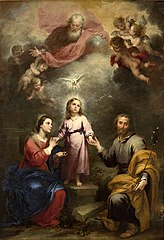
\includegraphics[scale=.5]{a20131222MeditationontheIncarnation-img001}
\end{wrapfigure}
Of its actuality, I am sure all readers are familiar with the story; if not, it is easy enough to find. There will be
objections to the story as miraculous and incredible, but these objections can only arise from an a priori commitment
to a positivist world view that cannot prove itself to be true. If, on the other hand, one is ready to accept the
actuality of unusual preternatural or supernatural phenomena, e.g., miraculous cures, amazing powers of yogis and
tulkus, the skills of magicians, etc., then the story of the birth of Jesus cannot be so easily rejected. There is only
the “vexed theological question of grace”, as Julius Evola called it in a recent translation; some will be willing to
see it, others will not.

However, in this meditation, we are not as interested in the Incarnation as a matter of faith, but rather as gnosis. We
will stipulate it as a given, and move on. As one of our mottos indicates, “truth lies in the interior of man” (St
Augustine). Augustine moved beyond Neoplatonism when he came to the realization that the Logos of the Greek
philosophers, understood in an objective and exterior way, was actually the same Logos Who was incarnated and is known
in man's interiority.

\paragraph{The Path of Affirmation}
This is expressed in the Path of Affirmation that is conceivable in the Incarnation. All previous forms of spirituality
follow the path of denial. Specifically, these would include Advaita Vedanta, Buddhism, and Neoplatonism. This path
ultimately tries to transcend the material conditions of life, including the human person, by the realization of
one's true identity as Brahman or the One. In this path, any determination is a limitation.

In the Path of Affirmation, on the contrary, God is approached through these determinations. St Athanasius describes the
Incarnation: Not by conversion of the Godhead into flesh, but by taking of the Manhood into God. This differs from
Oriental the idea of an Avatar in which a god takes on the appearance of a man for a specific purpose, e.g.,
Parashurama, an avatar of Vishnu, appeared to overcome the rule of the Kshatriyas.

Rather, the Logos raised the human up to God, once and for all. Christ, as the second Adam, restored the possibility of
the Primordial state to man. In this Path, man is not annihilated, so that only God remains, but instead there are two
who are united. Although largely ignored in common practice, this is an essential element of the catholic, apostolic,
Roman religion. Some quick examples, although many more can be found, including the official Catechism:

\textsc{Irenaeus}: The Word of God, our Lord Jesus Christ, who did, through His transcendent love, become what we are, that He
might bring us to be even what He is Himself.

\textsc{Clement of Alexandria}: The Word of God became man, that you may learn from man how man may become God.

Of course, the premier example of this teaching is Dante's Divine Comedy, where he shows us the
path to union with God through the rich imagery of his poetry.

In Christian Hermetism, particularly as evidenced in Valentin Tomberg\footnote{\url{https://www.meditationsonthetarot.com/the-elements-of-sacred-magic}} in our time, the birth of the Logos in
consciousness is the result of the alchemical marriage between the Holy Spirit and the purified soul. That becomes the
new, or absolute self, in union with the Father, or absolute being.

So, the goal of this path is the spiritual and alchemical transformation of man, and even the world. Ultimately, no one
can be convinced of this through any type of rational argument, so this is only an invitation to follow that path. Once
any type of realization of this nature is reached, one's faith is secure.

\paragraph{The World Process}
In the literature on tradition, most of the attention is focused on metaphysical teachings that aim to transcend all
material circumstances. There is lip service to social organization, viz., the idea of castes and hierarchy, as well as
the notion of cycles of the four ages. However, the relation of metaphysics to the world process is often left unclear;
to those who are striving to be liberated from all worlds, what difference would it make?

But, if the real path is the Path of Affirmation, then it does indeed make a difference. In the idea of the four ages,
there is often the misconception that the ages run according to some independent and objective cosmic clock. If that is
true, then one can be passive and simply wait for events to occur. In particular, the end of the Kali Yuga comes at the
prescribed moment apart from any consciousness of it. That is indeed odd for a teaching that regards consciousness as
primary over the physical and material. If that were true, then Guenon's call for the
establishment of a new elite would make no sense.

All traditions recognize three forces: the three gunas in the Vedanta, or the Great Triad of Taoism. We will stick to
the Western formulation of Providence, Will, and Destiny. Destiny is the automatic and deterministic element of the
world process. Its law is that of increasing entropy; left to its own devices, the world winds down, ultimately to a
totally undifferentiated state. This is compatible with profane science.

Of course, such a state is impossible, since nothing could occur in it and God is Infinite possibility. Providence is
God's or Heaven's influence on the process, not through force, but rather
through suggestion and persuasion.  This opens up new possibilities, especially the possibility for a new world to
follow the old when all its possibilities have been exhausted. The middle term in this is the Will of man, responding
to Providence and transforming his being and that of the world.

\paragraph{Creation and Redemption}
The pagan view of cycles was defective. It regarded the world as uncreated with no beginning and man as perpetual.
Hence, cycles reoccurred, in perpetual return, the same thing over and over. Even Guenon rejected this, since, in his
view, a world had a beginning and an end, the end of one being the beginning of another, much different, world.

This we take as closer to the truth. Hence, we must understand the cycle, from a perfect age to an ever more degenerate
one, and finally to the birth of a new age that is both in continuity with and different from its predecessor. This
must be understand as a drama involving God, man, and the earth, not as the predetermined result of a mindless process,
or even worse, some demiurge.

Hence, the transition from a golden age to a lesser one, did not happen according to some calendar, but was rather the
result of man's will. On the other side, the transition from the kali yuga to a golden age cannot
happen from within the world process but rather it must be interjected into it from a transcendent or providential
source, to then be adopted by the Will of man, at least by some who will be the leaven.

So the Incarnation is the beginning of the process of Redemption, that is, the regeneration of man and the world in a
world to come. That is why Valentin Tomberg could regard Creation and Redemption as the two great magical acts since
magic “requires the perfect union in Love between two distinct and free wills: the divine and the human”.

We know creation interiorly through the memory of the Primordial state and its loss. There is the testimony of saints
and mystics, there is the evidence of it through perduring vestigial preternatural powers of the soul; ultimately,
conviction comes through our own remembrance of that state.

Similarly, for the Incarnation. We know that there have been saints who have reached the divine union, or Beatific
Vision, in this life, the Western equivalent of the jivan-mukti. We, too, may have been graced with a taste of that
union.

A follow up will deal with the scientific and metaphysical issues involved with this.

\flright{\itshape Posted on 2013-12-22 by Cologero}

\begin{center}* * *\end{center}

\begin{footnotesize}\begin{sffamily}
\hfill

\texttt{JA on 2013-12-23 at 10:22 said: }

Gnosis is not heresy, heresy is denial of the true facts as given in the Creed and as taught by the Councils and the
Magisterium. Gnosticism denies Christ came in the flesh.

Catholicism is an elitist religion, read the book Nobility by Dr Plinio if you doubt that.

“taste of union”... so Cologero, you have achieved theosis ?

Blessed Christmas, my brother in Christ !

\hfill

\texttt{scardanelli on 2013-12-23 at 10:25 said: }

“Ultimately, no one can be convinced of this through any type of rational argument, so this is only an invitation to
follow that path.”

In the previous posts on Evola and Coue, we have seen that Faith is certainly a necessary begining condition. Yet
ultimately faith must be resolved in certainty. What the discursive mind believes upon faith must be seen and verified
within. When one sees the truth in this fashion, there is no more need to argue or attack the assertions of others. One
can perform spiritual works of mercy out of love for ones neighbor though. 

When Faith stagnates, when it is not resolved in certainty, it becomes rigid dogma, it becomes the empty worship of the
Pharisees. Thus one feels the need to “protect” the truth, when in reality, the truth is and always will remain without
your help. Certainty from within is the way to spiritualize matter and to establish truth in the midst of this world.
This is the ultimate support of Orthodoxy.

\hfill

\texttt{Matt on 2013-12-24 at 11:42 said: }

No talk of the act of creation being fundamentally misguided and/or evil, no talk of the world being created by a
being/principle opposed to the True God; I fail to see how the post is gnostic in the historical-religous sect sense,
nor do I see a supposed initiatic fetishism.

Merry Christmas.

\hfill

\texttt{Jacob on 2013-12-24 at 21:58 said: }

I try to avoid posts that contain just praises, but this was was such a great post IMO. The comments were very
interesting a well. There did not seem to be anything Gnostic in the post to me. In fact, as Cologero said the
Clementine initiation post is a great post on Gnosticism. Still, I think even things connected to Gnosticism are useful
insights as long as they can be separated from the specifically heretical teachings. I mean, I
don't think anyone who is actually informed on these things would say using Meister
Eckhart's teachings are a bad idea, although he ran into trouble with ye inquisition. The Templars
and the Jesuits as well had their problems. 

Anyway, Merry Christmas everyone.

\hfill

\texttt{Michael on 2013-12-24 at 22:00 said: }

I've been wondering how Tomberg's path relates to
Guenon's idea of the elite. Thank you for clarifying. Those who follow the path outlined by
Tomberg are those who cooperate with the providential spark (“Thy will be done”) that will bring about the golden age.

It seems that Catholicism is both exoteric and esoteric at the same time, and the esoteric can be uncovered by those who
approach from both a hermetic or exoteric angle.

Merry Christmas!

\hfill

\texttt{anon on 2013-12-25 at 10:15 said: }

Speaking of Gnosticism, not only as historical sect, but primarily as an eternal tendency (or current) within the human
heart, either dormant or active, one that occurs in the context of many religious different traditions, and which finds
not only spiritual, but also political expression, I was glad to see two articles on Gornahoor that mention Voegelin. I
stumbled across him before ever hearing about Evola or Guenon.

\begin{quotationx}\scriptsize

The death of the spirit is the price of progress. Nietzsche revealed this mystery of the Western apocalypse when he
announced that God was dead and that He had been murdered. This Gnostic murder is constantly committed by the men who
sacrificed God to civilization. The more fervently all human energies are thrown into the great enterprise of salvation
through world–immanent action, the farther the human beings who engage in this enterprise move away from the life of
the spirit. And since the life the spirit is the source of order in man and society, the very success of a Gnostic
civilization is the cause of its decline.

A civilization can, indeed, advance and decline at the same time—but not forever. There is a limit
toward which this ambiguous process moves; the limit is reached when an activist sect which represents the Gnostic
truth organizes the civilization into an empire under its rule. Totalitarianism, defined as the existential rule of
Gnostic activists, is the end form of progressive civilization.

– Eric Voegelin

\hfill

“One comment I should make right now. Obviously the title `Gnosticism and
Modernity' is, at least partly, inspired by my own work in the field. But when I hit on this
problem, that was 25 years ago. In the meantime, science in this matter has advanced. And today I would have to say
that Gnosticism is one component in the historical structure of modernity but no more than one.”

– Eric Voegelin

\hfill

“I have been called every conceivable name by partisans of this or that ideology… a Communist, a Fascist, a National
Socialist, an old liberal, a new liberal, a Jew, a Catholic, a Protestant, a Platonist, a neo-Augustinian, a Thomist,
and of course a Hegelian.”

– Eric Voegelin

\end{quotationx}

\hfill

\texttt{Michel on 2013-12-26 at 16:02 said: }
\begin{flushleft}
Oh that with yoke tender,

Realize thy burden great bull,

Plough thine fields strangely,

With the fierceness of a thousand suns,

Subtly dancing to finer hymns,

Pouring as gentle streams from breaking skies,

Arise thou Great Morning Star!

Seize thy rightful place stolen from thee,

Fly thou blithe spirit, in swirls of liquid burning,

Embrace The Son of like particle,

Ever galvanized, progenitor of Thee once silent,

Now e'er flaring Blazing Song.
\end{flushleft}

\hfill

\texttt{Cologero on 2013-12-27 at 00:17 said: }

I have been away visiting family and am just now catching up on comments, for whose civilized tone and intelligence I am
grateful, even those who respectfully disagree. Of course, I have no desire to be “original”; rather, I want only to
bring to light what has been forgotten and perhaps re-express it in contemporary terms. If anyone is still confused by
this post, please ponder these words from St Augustine (Confessions, Book XI, Ch 8):

\begin{quotex}\scriptsize
Thus, in the gospel He speaks through the flesh; and this sounded outwardly in the ears of men, that it might be
believed and sought inwardly, and that it might be found in the eternal Truth, where the good and only Master teaches
all His disciples. 

\end{quotex}

\hfill

\texttt{Max on 2013-12-27 at 17:36 said: }

A child might live happily without worries, almost not even conscious of himself. But he still wishes to grow up, know and do things. We must not necessarily regard the processsion of the ages of the world as a degeneration. It depends on perspective. Through the different qualities of time we can know the whole like a child gets to know himself as he grows older. If as an old man he still remembers how it is to be a child in his heart, he is beyond time and can see all in a single instant. There is a purpose to living which can only be found and fullfilled by living.

\hfill

\end{sffamily}\end{footnotesize}